\documentclass[14pt]{extarticle}

\usepackage{projectstemplate}
\usepackage[askip=3mm, bskip=3mm]{terminal}
\usepackage[askip=3mm, bskip=3mm]{mylisting}
\usepackage{tikz}
\usetikzlibrary{positioning, shapes.geometric}
\usepackage{csquotes}

\title{Задание проекта \\ "Библиотека идентификации и аутентификации"}

\begin{document}

\maketitle

\tableofcontents

\clearpage

\section{Термины и определения}

\begin{itemize}

 \item \textbf{Идентификация} --- поиск учетной записи пользователя в базе
  данных по переданным учетным данным. 
  Чаще всего для поиска используется логин или имя пользователя.

 \item \textbf{Аутентификация} --- подтверждение подлинности пользователя
  по переданным учетным данным.
  Чаще всего для этого проверяется пароль пользователя.

 \item \textbf{Хэш-сумма (хэш)} --- массив данных фиксированной длины, который
  получается из другого массива данных произвольной длины при помощи алгоритма
  хэширования.
  Любое изменение в исходном массиве данных влияет на хэш-сумму.

 \item \textbf{Криптографическая хэш-сумма} --- хэш-сумма, полученная в
  при помощи одного из криптографически стойких алгоритмов хэширования.
  Одним из свойств таких алгоритмов является необратимость преобразования:
  невозможно получить массив исходных данных, зная только его хэш.
  Такие хэш-суммы широко используются для хранения паролей в базах данных.
  В таких случаях, в базе данных вместо пароля хранится его хэш.
  При аутентификации пользователя вычисляется хэш полученного от него пароля
  и сравнивается с эталонным в базе данных.

  Одним из примеров криптографически стойких алгоритмов хэширования является
  SHA256\footnotemark{}.

  \footnotetext{\url{https://ru.wikipedia.org/wiki/SHA-2}}

 \item \textbf{Соль} --- массив данных, который используется в
  алгоритме хэширования для вычисления хэша.
  Можно считать, что хэш-преобразование выполняется над некоторой комбинацией
  массива исходных данных и соли, например, над результатом их конкатенации
  (присоединения друг к другу).
  Существуют и более сложные механизмы комбинации соли и массива исходных
  данных.
  Один из них определяет стандарт PBKDF2\footnotemark{}.

  \footnotetext{\url{https://en.wikipedia.org/wiki/PBKDF2}}
  
  Необходима для усложнения криптоанализа злоумышленником в случае утечки
  базы данных.
  Часто пользователи используют не очень сложные пароли (например,
  \textit{12345678}), и у злоумышленника появляется возможность перебрать
  самые распространенные варианты, вычислить их хэш-суммы и сравнить их с хэшами
  в базе данных\footnotemark{}.
  Чем больше в базе данных учетных записей пользователей, тем выше шанс, что
  вычисленный хэш совпадет с каким-нибудь эталонным хэшем из базы.
  Если \enquote{солить} хэши, то злоумышленнику для взлома базы перебором необходимо
  будет так же знать и соль.

  \footnotetext{\url{https://en.wikipedia.org/wiki/Dictionary_attack}}

 \item \textbf{Динамическая соль} --- соль, которая генерируется для каждого
  входного массива данных индивидуально.
  При таком подходе для одного и того же пароля получаются разные хэш-суммы,
  что затрудняет криптоанализ базы данных.
  Криптоаналитику не удается установить факт использования одинакового пароля
  разными пользователями.
  При таком подходе допускается хранение соли вместе с хэш-суммами паролей
  в той же базе данных.

\end{itemize}

\section{Задание}

\subsection{Общие сведения о системе}

Это задание предлагает для разработки систему, которую можно проиллюстрировать
схемой на рис.~\ref{fig:scheme}.

\begin{figure}[h!]
 \centering
 \begin{tikzpicture}[
  box/.style={draw, minimum width=3.5cm, minimum height=5cm},
  innerbox/.style={draw, dashed, minimum width=2.5cm, minimum height=1.5cm},
  db/.style={cylinder, cylinder uses custom fill, cylinder body fill=white,
             draw, shape border rotate=90, aspect=0.5, minimum height=1cm,
             minimum width=1cm},
  font=\small
 ]

  % ПК блок
  \node[box] (pc) {};
  \node[above=0.2cm of pc] {ПК};
  \node[innerbox, above=0.7cm of pc.south] (driver) {Драйвер};
  \node[anchor=north, inner sep=0pt] at ([yshift=-0.5cm,xshift=1.8cm]pc.north west) 
   {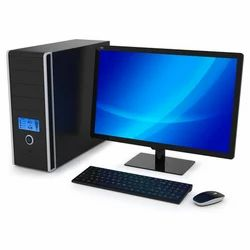
\includegraphics[width=1.5cm]{pc.jpg}};

  % Контроллер блок
  \node[box, right=3cm of pc] (ctrl) {};
  \node[above=0.2cm of ctrl] {Контроллер};
  \node[db, above=1.4cm of ctrl.south] (db) {};
  \node[align=center, below=0.1cm of db] {База данных\\пользователей};
  \node[anchor=north, inner sep=0pt] at ([yshift=-0.5cm,xshift=1.8cm]ctrl.north west) 
   {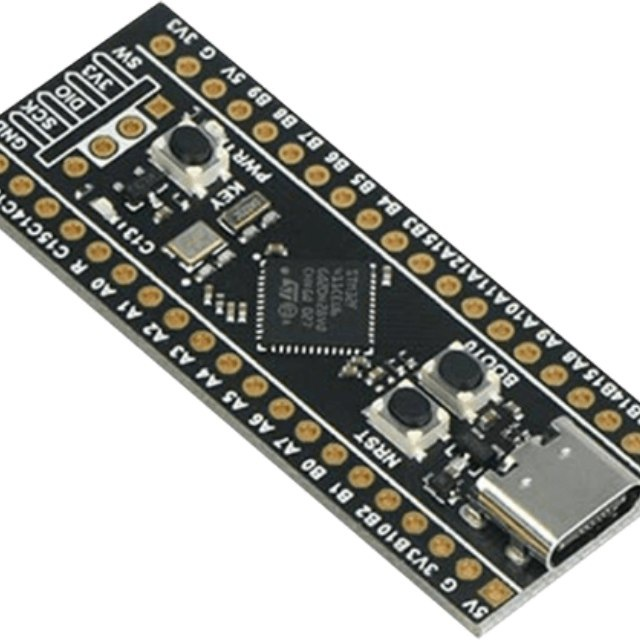
\includegraphics[width=1.5cm]{blackpill.jpg}};

  % Соединение USB
  \draw[-] (pc.east) -- (ctrl.west) node[midway, above] {USB};
  \fill (pc.east) circle (2pt);
  \fill (ctrl.west) circle (2pt);
 \end{tikzpicture}
 \caption{Схема системы}\label{fig:scheme}
\end{figure}

Компоненты системы:

\begin{itemize}
 \item{\textbf{Контроллер}} --- устройство STM32F411CEU6 (WeAct BlackPill 2.0).
  ПО контроллера обрабатывает команды, приходящие по USB, и отправляет ответ на
  них.
 \item{\textbf{База данных пользователей}} --- хранилище учетных данных пользователей
  в энерегонезависимой памяти (Flash) контроллера.
  Его наполнение может меняться при обработке некоторых команд, которые обрабатывает
  ПО контроллера.
 \item{\textbf{ПК}} --- персональный компьютер, выступающий в роли клиента
  контроллера.
  С ПК контроллеру по USB отправляются команды.
 \item{\textbf{Драйвер}} --- ПО, предназначенное для отправки команд контроллеру и
  взаимодействия с пользователем ПК.
  Драйвер получает команду от пользователя, сериализует ее, отправляет контроллеру,
  читает ответ и представляет его пользователю в человекочитаемом виде.
\end{itemize}

Контроллер и драйвер вазимодействуют с помощью команд.
Инициатором обмена и отправителем команды всегда является драйвер.
После обработки команды контроллер обязан отправить драйверу ответ.

\subsection{Функциональные требования}

\subsubsection{Команды}

Задание определяет набор команд и их аргументы, конкретное представление команд
в памяти контроллера и в среде обмена определяется реализацией.

ПО контроллера должно отвечать на каждую команду.
Ответ должен по меньшей мере содержать результат выполнения команды (успешно
или неуспешно).
Ответ может (но не обязан) содержать причину неудачи выполнения команды.

Ниже приведен список, которые должны поддерживать драйвер и контроллер.
Команды приведены в нотации

\begin{center}
 \texttt{\textbf{command <argument> <argument>...}},
\end{center}

в которой \texttt{\textbf{command}} --- имя команды, а \texttt{\textbf{argument}}
--- её аргумент.

\begin{enumerate}

 \item \texttt{\textbf{auth <login> <password>}}

 Команда идентификации и аутентификации.
 Контроллер должен возвращать ответ ``успешно'', если пользователь с именем
 \texttt{\textbf{login}} существует и его пароль \texttt{\textbf{password}} прошел
 проверку.

 \item \texttt{\textbf{users}}

 Команда для получения списка пользователей.
 Контроллер должен ответить списком имен пользователей из базы данных.

 \item \texttt{\textbf{changepassword <login> <old\_password> <new\_password>}}

 Команда для смены пароля пользователя.
 Если по учетным данным \texttt{\textbf{login}} и \texttt{\textbf{old\_password}}
 удалось идентифицировать и аутентифицировать пользователя, то контроллер должен
 обновить пароль пользователя в базе на \texttt{\textbf{new\_password}} и вернуть
 ответ ``успешно''.

 \item \texttt{\textbf{adduser <password> <user\_login> <user\_password>}}

 Команда для добавления нового пользователя.
 Если пароль \texttt{\textbf{password}} подходит встроенной учетной записи
 с именем ``admin'', и учетной записи с именем \texttt{\textbf{user\_login}}
 не существует, то контроллер должен добавить в базу нового пользователя
 с учетными данными \texttt{\textbf{user\_login}} и \texttt{\textbf{user\_password}} 
 и вернуть ответ ``успешно''.

 \item \texttt{\textbf{deluser <password> <user\_login>}}

 Команда для удаления пользователя.
 Если пароль \texttt{\textbf{password}} подходит встроенной учетной записи
 с именем ``admin'', учетная запись с именем \texttt{\textbf{user\_login}}
 существует и это не учетная запись встроенного пользователя ``admin''',
 то контроллер должен должен удалить из базы пользователя с этим именем
 и вернуть ответ ``успешно''.
 
\end{enumerate}

\subsubsection{ПО контроллера}

\begin{enumerate}

 \item База данных пользователей должна храниться в энергонезависимой
  памяти устройства.

 \item После установки ПО на контроллер в базе должна быть только учетная запись
  пользователя ``admin'' с логином \textit{admin} и одноразовым паролем
  \textit{admin}.

 \item После установки ПО на контроллер его ПО должно отказывать в выполнении
  любой команды, кроме \texttt{\textbf{changepassword admin <password>}}.
  До смены одноразового пароля учетной записи ``admin'' контроллер считается не
  сконфигурированным.

\end{enumerate}

\subsubsection{Драйвер}

\begin{enumerate}

 \item Драйвер должен принимать команды в человекочитаемом виде (из потока
  ввода или из файла) и преобразовывать их во внутреннее представление, работать
  с которым может он сам и ПО контроллера.

 \item Драйвер должен предоставлять пользователю ответ в человекочитаемом виде.

\end{enumerate}

\subsection{Нефункциональные требования}

\begin{enumerate}

 \item Базы данных пользователей должно быть достаточно для хранения минимум
  10 пользователей.

 \item Пароль должен состоять из символов [a-Z0-9].

 \item Длина имени пользователя и пароля не должны превышать 20 символов.

 \item При получении некорректной команды контроллер не должен изменять
  наполнение базы данных.

 \item ПО контроллера должно быть устойчиво к ошибкам сегментации, выхода за
  границы массива и т.д.

\end{enumerate}

\subsection{Требования информационной безопасности}

\begin{enumerate}

 \item Пароли пользователей не должны храниться в базе данных в открытом виде.
  Вместо этого в базе данных должны храниться в хэши паролей.

 \item Для хэширования паролей должна использоваться динамическая соль.
  Соль допускается хранить в базе данных пользователей.

 \item Контроллер должен быть устойчив к атакам отказа в доступе (DoS), т.е.
  никакая команда не должна приводить к тому, что контроллер больше не будет
  обрабатывать следующие команды.

\end{enumerate}

\section{Рекомендации по выполнению}

\begin{enumerate}

 \item В качестве шаблона проекта ПО контроллера возьмите
  \href{https://github.com/czertyaka/blackpill-usb-sha256}{этот репозиторий}.

 \item Продумайте внутреннее представление команд и ответов.
  Командам и символам можно назначить кодировки, уменьшив таким образом размер
  пакетов обмена между драйвером и контроллером.

 \item Для хэширования рекомендуется использовать алгоритм PBKDF2\footnotemark{}.

 \footnotetext{\url{https://www.wolfssl.com/documentation/manuals/wolfssl/group\_\_Password.html\#function-wc\_pbkdf2}}

 \item Для вычисления динамической соли используйте генератор рандомных чисел\footnotemark{}.

 \footnotetext{\url{https://www.wolfssl.com/documentation/manuals/wolfssl/group\_\_Random.html\#function-wc\_rng\_generateblock}}

 \item По возможности избегайте динамической аллокации памяти.

 \item Распределите роли между участниками проекта: кто-то должен заниматься
  разработкой драйвера, кто-то ПО контроллера, кто-то системами сборки, тестированием,
  отчетом и т.д.

\end{enumerate}

\end{document}
